\def\bmode{2} % Mode 0 for presentation, mode 1 for a handout with notes, mode 2 fo% r handout without notes
\if 0\bmode
\documentclass[usenames,dvipsnames,smaller, hyperref={colorlinks=true,urlcolor=magenta,citecolor=cyan,linkcolor=orange}]{beamer}
\else \if 1\bmode
\immediate\write18{pdflatex -jobname=\jobname-Handout-Notes\space\jobname}
\documentclass[usenames,dvipsnames,smaller,handout,hyperref={colorlinks=true,urlcolor=magenta,citecolor=cyan,linkcolor=orange}]{beamer}
\usepackage{handoutWithNotes}
\pgfpagesuselayout{2 on 1 with notes}[letterpaper, landscape, border shrink=4mm]
\else \if 2\bmode
\immediate\write18{pdflatex -jobname=\jobname-Handout\space\jobname}
\documentclass[usenames,dvipsnames,smaller,handout,hyperref={colorlinks=true,urlcolor=magenta,citecolor=cyan,linkcolor=orange}]{beamer}
\fi
\fi
\fi


% \documentclass[smaller,handout
% ]{beamer}
%\usepackage{etex}
%\newcommand{\num}{6{} }

% \usetheme[
%   outer/progressbar=foot,
%   outer/numbering=counter,
%  block=fill
% ]{metropolis}

%\useoutertheme{metropolis}

\usetheme{Madrid}
\useoutertheme[subsection=false]{miniframes} % Alternatively: miniframes, infolines, split
\useinnertheme{circles}
\usecolortheme{seahorse}

\usepackage[backend=biber,style=authoryear,maxcitenames=2,maxbibnames=99,safeinputenc,url=false,
eprint=false]{biblatex}
\addbibresource{bib/references.bib}
\AtEveryCitekey{\iffootnote{{\tiny}\tiny}{\tiny}}

%\usepackage{pgfpages}
%\setbeameroption{hide notes} % Only slides
%\setbeameroption{show only notes} % Only notes
%\setbeameroption{hide notes} % Only notes
%\setbeameroption{show notes on second screen=right} % Both

% \usepackage[sfdefault]{Fira Sans}

% \setsansfont[BoldFont={Fira Sans}]{Fira Sans Light}
% \setmonofont{Fira Mono}

%\usepackage{fira}
%\setsansfont{Fira}
%\setmonofont{Fira Mono}
% To give a presentation with the Skim reader (http://skim-app.sourceforge.net) on OSX so
% that you see the notes on your laptop and the slides on the projector, do the following:
% 
% 1. Generate just the presentation (hide notes) and save to slides.pdf
% 2. Generate onlt the notes (show only nodes) and save to notes.pdf
% 3. With Skim open both slides.pdf and notes.pdf
% 4. Click on slides.pdf to bring it to front.
% 5. In Skim, under "View -> Presentation Option -> Synhcronized Noted Document"
%    select notes.pdf.
% 6. Now as you move around in slides.pdf the notes.pdf file will follow you.
% 7. Arrange windows so that notes.pdf is in full screen mode on your laptop
%    and slides.pdf is in presentation mode on the projector.

% Give a slight yellow tint to the notes page
%\setbeamertemplate{note page}{\pagecolor{yellow!5}\insertnote}\usepackage{palatino}


%\usetheme{metropolis}
%\usecolortheme{beaver}
%\usepackage{xcolor}
\definecolor{darkcandyapplered}{HTML}{A40000}
\definecolor{lightcandyapplered}{HTML}{e74c3c}

%\setbeamercolor{title}{fg=darkcandyapplered}
%\setbeamercolor{frametitle}{bg=darkcandyapplered!80!black!90!white}
%\setbeamertemplate{frametitle}{\bf\insertframetitle}
%\setbeamercolor{footnote mark}{fg=darkcandyapplered}
%\setbeamercolor{footnote}{fg=darkcandyapplered!70}
%\Raggedbottom
%\setbeamerfont{page number in head/foot}{size=\tiny}
%\usepackage[tracking]{microtype}


\setbeamertemplate{frametitle}{%
    \nointerlineskip%
    \begin{beamercolorbox}[wd=\paperwidth,ht=2.0ex,dp=0.6ex]{frametitle}
        \hspace*{1ex}\insertframetitle%
    \end{beamercolorbox}%
}



\setbeamerfont{caption}{size=\footnotesize}
\setbeamercolor{caption name}{fg=darkcandyapplered}


%\usepackage[sc,osf]{mathpazo}   % With old-style figures and real smallcaps.
%\linespread{1.025}              % Palatino leads a little more leading

% Euler for math and numbers
%\usepackage[euler-digits,small]{eulervm}
%\AtBeginDocument{\renewcommand{\hbar}{\hslash}}
\usepackage{graphicx,multirow,paralist,booktabs}


%\mode<presentation> { \setbeamercovered{transparent} }

\setbeamertemplate{navigation symbols}{}
\makeatletter
\def\beamerorig@set@color{%
  \pdfliteral{\current@color}%
  \aftergroup\reset@color
}
\def\beamerorig@reset@color{\pdfliteral{\current@color}}
\makeatother

%=== GRAPHICS PATH ===========
\graphicspath{{./m3-images/}}
% Marginpar width
%Marginpar width
%\setlength{\marginparsep}{.02in}


%% Captions
% \usepackage{caption}
% \captionsetup{
%   labelsep=quad,
%   justification=raggedright,
%   labelfont=sc
% }

%AMS-TeX packages

\usepackage{amssymb,amsmath,amsthm} 
\usepackage{bm}
\usepackage{color}

\usepackage{hyperref,enumerate}
\usepackage{minitoc,array}


%https://tex.stackexchange.com/a/31370/2269
\usepackage{mathtools,cancel}

\renewcommand{\CancelColor}{\color{red}} %change cancel color to red

\makeatletter
\let\my@cancelto\cancelto %copy over the original cancelto command
\newcommand<>{\cancelto}[2]{\alt#3{\my@cancelto{#1}{#2}}{\mathrlap{#2}\phantom{\my@cancelto{#1}{#2}}}}
% redefine the cancelto command, using \phantom to assure that the
% result doesn't wiggle up and down with and without the arrow
\makeatother


\definecolor{slblue}{rgb}{0,.3,.62}
\hypersetup{
    colorlinks,%
    citecolor=blue,%
    filecolor=blue,%
    linkcolor=blue,
    urlcolor=slblue
}

%%%TIKZ
\usepackage{tikz}
\usepackage{pgfplots}
\usepackage{pgfplotstable}
\usepackage{pgfgantt}
\usepackage{tikzsymbols}
\pgfplotsset{compat=newest}

\usetikzlibrary{arrows,shapes,positioning,shapes.geometric}
\usetikzlibrary{decorations.markings}
\usetikzlibrary{shadows,automata}
\usetikzlibrary{patterns}
\usetikzlibrary{trees,mindmap,backgrounds}
%\usetikzlibrary{circuits.ee.IEC}
\usetikzlibrary{decorations.text}
% For Sagnac Picture
\usetikzlibrary{%
    decorations.pathreplacing,%
    decorations.pathmorphing%
}
\tikzset{no shadows/.style={general shadow/.style=}}
%
%\usepackage{paralist}


%%% FORMAT PYTHON CODE
%\usepackage{listings}
% Default fixed font does not support bold face
\DeclareFixedFont{\ttb}{T1}{txtt}{bx}{n}{8} % for bold
\DeclareFixedFont{\ttm}{T1}{txtt}{m}{n}{8}  % for normal

% Custom colors
\definecolor{deepblue}{rgb}{0,0,0.5}
\definecolor{deepred}{rgb}{0.6,0,0}
\definecolor{deepgreen}{rgb}{0,0.5,0}

%\usepackage{listings}

% Python style for highlighting
% \newcommand\pythonstyle{\lstset{
% language=Python,
% basicstyle=\footnotesize\ttm,
% otherkeywords={self},             % Add keywords here
% keywordstyle=\footnotesize\ttb\color{deepblue},
% emph={MyClass,__init__},          % Custom highlighting
% emphstyle=\footnotesize\ttb\color{deepred},    % Custom highlighting style
% stringstyle=\color{deepgreen},
% frame=tb,                         % Any extra options here
    % showstringspaces=false            % 
% }}

% % Python environment
% \lstnewenvironment{python}[1][]
% {
% \pythonstyle
% \lstset{#1}
% }
% {}

% % Python for external files
% \newcommand\pythonexternal[2][]{{
% \pythonstyle
% \lstinputlisting[#1]{#2}}}

% Python for inline
% 
% \newcommand\pythoninline[1]{{\pythonstyle\lstinline!#1!}}


\newcommand{\osn}{\oldstylenums}
\newcommand{\dg}{^{\circ}}
\newcommand{\lt}{\left}
\newcommand{\rt}{\right}
\newcommand{\pt}{\phantom}
\newcommand{\tf}{\therefore}
\newcommand{\?}{\stackrel{?}{=}}
\newcommand{\fr}{\frac}
\newcommand{\dfr}{\dfrac}
\newcommand{\ul}{\underline}
\newcommand{\tn}{\tabularnewline}
\newcommand{\nl}{\newline}
\newcommand\relph[1]{\mathrel{\phantom{#1}}}
\newcommand{\cm}{\checkmark}
\newcommand{\ol}{\overline}
\newcommand{\rd}{\color{red}}
\newcommand{\bl}{\color{blue}}
\newcommand{\pl}{\color{purple}}
\newcommand{\og}{\color{orange!90!black}}
\newcommand{\gr}{\color{green!40!black}}
\newcommand{\nin}{\noindent}
\newcommand{\la}{\lambda}
\renewcommand{\th}{\theta}
\newcommand{\al}{\alpha}
\newcommand{\G}{\Gamma}
\newcommand*\circled[1]{\tikz[baseline=(char.base)]{
            \node[shape=circle,draw,thick,inner sep=1pt] (char) {\small #1};}}

\newcommand{\bc}{\begin{compactenum}[\quad--]}
\newcommand{\ec}{\end{compactenum}}

\newcommand{\p}{\partial}
\newcommand{\pd}[2]{\frac{\partial{#1}}{\partial{#2}}}
\newcommand{\dpd}[2]{\dfrac{\partial{#1}}{\partial{#2}}}
\newcommand{\pdd}[2]{\frac{\partial^2{#1}}{\partial{#2}^2}}



%%%%%%%%%%%%%%%%%%%%%%%%%%%%%%%%%%%%%%%%%%%%%%%%%%%
%%%%%%%%%%%%%%%%%%%%%%%%%%%%%%%%%%%%%%%%%%%%%%%%%%%

\title[CEE 260/MIE 273 3a: Random Variables]{{\normalsize CEE 260/MIE 273: Probability and Statistics in Civil Engineering} \\
Lecture 3a: Introduction: Random variables}
\date[\today]{\footnotesize \today}
\author{{\bf Prof.\ Oke}}
\institute[UMass Amherst]{
  \begin{tikzpicture}[baseline=(current bounding box.center)]
    \node[anchor=base] at (-7,0) (its) {
\includegraphics[scale=.3]{UMassEngineering_vert}} ;
  \end{tikzpicture}
}



%https://tex.stackexchange.com/questions/55806/mindmap-tikzpicture-in-beamer-reveal-step-by-step
  % \tikzset{
  %   invisible/.style={opacity=0},
  %   visible on/.style={alt={#1{}{invisible}}},
  %   alt/.code args={<#1>#2#3}{%
  %     \alt<#1>{\pgfkeysalso{#2}}{\pgfkeysalso{#3}} % \pgfkeysalso doesn't change the path
  %   },
  % }


\usepackage{listings}

\lstset{language=matlab,
                basicstyle=\scriptsize\ttfamily,
                keywordstyle=\color{blue}\ttfamily,
                stringstyle=\color{blue}\ttfamily,
                commentstyle=\color{gray}\ttfamily,
                morecomment=[l][\color{gray}]{\#}
              }
         
\begin{document}

\maketitle




\begin{frame}
  \frametitle{M2c Recap: Conditional Probability and Bayes' Theorem}
   \begin{itemize}[<+->]
  \item Total probability:
    \begin{equation}
      P(A) = P(A|E_{1})P(E_{1}) + P(A|E_{2})P(E_{2}) + \cdots + P(A|E_{n})P(E_{n})
    \end{equation}

  \item Bayes' Theorem for two events: \pause
    \begin{equation}
      P(B|A) = \fr{P(A|B)P(B)}{P(A)}
    \end{equation}
    \pause
    For multiple events: \pause 
    \begin{eqnarray}
      P(E_{1}|A) &=& \fr{P(A|E_{1})P(E_{1})}{\bl  P(A|E_{1})P(E_{1}) + P(A|E_{2})P(E_{2}) + \cdots + P(A|E_{n})P(E_{n})}\\[2mm] \pause
      &=&  \fr{P(A|E_{1})P(E_{1})}{\bl  P(A)}
    \end{eqnarray}

  \end{itemize}
\end{frame}

\begin{frame}
  \frametitle{Overview of Module 3}
  \pause
  Overview
  \begin{itemize}
  \item Lecture 3a:  Introduction: Random Variables \pause
  \item Lecture 3b: Normal Distribution \pause 
  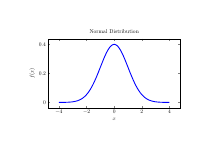
\begin{tikzpicture}[
    scale=.2]
    \begin{axis}[
        width=10cm, height=6cm,
        xlabel=$x$,
        ylabel=$f(x)$,
        title={Normal Distribution},
        samples=100,
        domain=-4:4
    ]
    % Standard Normal (μ=0, σ=1)
    \addplot[blue,ultra  thick] {exp(-(x^2)/2)/sqrt(2*pi)};
    \end{axis}
\end{tikzpicture}
  \item Lecture 3c: Lognormal  \pause
  % Lognormal Distribution
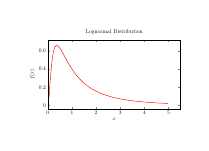
\begin{tikzpicture}[scale=.2]
    \begin{axis}[
        width=10cm, height=6cm,
        xlabel=$x$,
        ylabel=$f(x)$,
        title={Lognormal Distribution},
        samples=100,
        domain=0:5,
        xmin=0
    ]
    % μ=0, σ=1
    \addplot[red, thick] {exp(-(ln(x))^2/2)/(x*sqrt(2*pi))};
    \end{axis}
\end{tikzpicture} \pause and Exponential Distributions \pause
  % Exponential Distribution
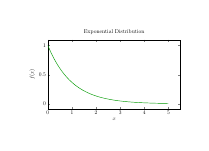
\begin{tikzpicture}[scale=.2]
    \begin{axis}[
        width=10cm, height=6cm,
        xlabel=$x$,
        ylabel=$f(x)$,
        title={Exponential Distribution},
        samples=100,
        domain=0:5,
        xmin=0
    ]
    % λ=1
    \addplot[green!60!black, thick] {exp(-x)};
    \end{axis}
\end{tikzpicture}
  \item Lecture 3d: Binomial Distribution \pause 
\begin{tikzpicture}[scale=.2]
    \begin{axis}[
        width=10cm, height=6cm,
        xlabel=$k$,
        ylabel=$P(X=k)$,
        title={Binomial Distribution},
        ybar,
        xtick=data,
        symbolic x coords={0,1,2,3,4,5,6,7,8,9,10},
        enlarge x limits=0.2
    ]
    % n=10, p=0.5
    \addplot[blue, fill] coordinates {
        (0,0.001)
        (1,0.010)
        (2,0.044)
        (3,0.117)
        (4,0.205)
        (5,0.246)
        (6,0.205)
        (7,0.117)
        (8,0.044)
        (9,0.010)
        (10,0.001)
    };
    \end{axis}
\end{tikzpicture}
  \item Lecture 3e: Poisson Distribution \pause
                                                                              \begin{tikzpicture}[scale=.2]
    \begin{axis}[
        width=10cm, height=6cm,
        xlabel=$k$,
        ylabel=$P(X=k)$,
        title={Poisson Distribution},
        ybar,
        xtick=data,
        nodes near coords=false,
        bar width=6pt,
        symbolic x coords={0,1,2,3,4,5,6,7,8},
        enlarge x limits=0.2
    ]
    % λ=3
    \addplot[red, fill] coordinates {
        (0,0.050)
        (1,0.149)
        (2,0.224)
        (3,0.224)
        (4,0.168)
        (5,0.101)
        (6,0.050)
        (7,0.022)
        (8,0.008)
    };
    \end{axis}
\end{tikzpicture}
  \item Lecture 3f: Joint Distributions and further topics
  \end{itemize}
\end{frame}


\begin{frame}
  \frametitle{Objectives and outline}
  \pause

  \begin{itemize}[<+->]
  \item Understand random variables

  \item Distinguish between discrete and continuous random variables
    
  \item Compute measures of centrality and dispersion, as well as sketch PMFs, PDFs and CDFs
  \end{itemize}
  \pause
    \tableofcontents


\end{frame}


\section{Introduction to random variables}
\begin{frame}
  \frametitle{Random variables}\pause

  \begin{block}{Definitions}
    \begin{itemize}

    \item A random variable (r.v.) represents the values of the outcomes in a sample space \pause (e.g. the outcome of die roll: $X = \{1, 2, 3, 4, 5, 6 \}$ \pause
    \item A random variable is a function that uniquely maps events in a sample space to the set of real numbers. 
\end{itemize}

\end{block}


  A random variable $X$ may be: \pause

  \begin{itemize}
  \item {\it Discrete}
  \item {\it Continuous}
  \end{itemize}
  
\end{frame}


\begin{frame}
  \frametitle{Describing random variables}
  \pause

  \begin{block}{Central values}
    \begin{itemize}[<+->]
    \item Mean
    \item Median
    \item Mode
    \end{itemize}
  \end{block}

  \pause

  \begin{block}{Measures of dispersion}
    \begin{itemize}[<+->]
    \item Variance
    \item Standard deviation
    \item Coefficient of variation (COV)
    \end{itemize}
  \end{block}
\end{frame}

% \begin{frame}
%   \frametitle{Population versus sample}
%   \pause

%   \begin{center}
%     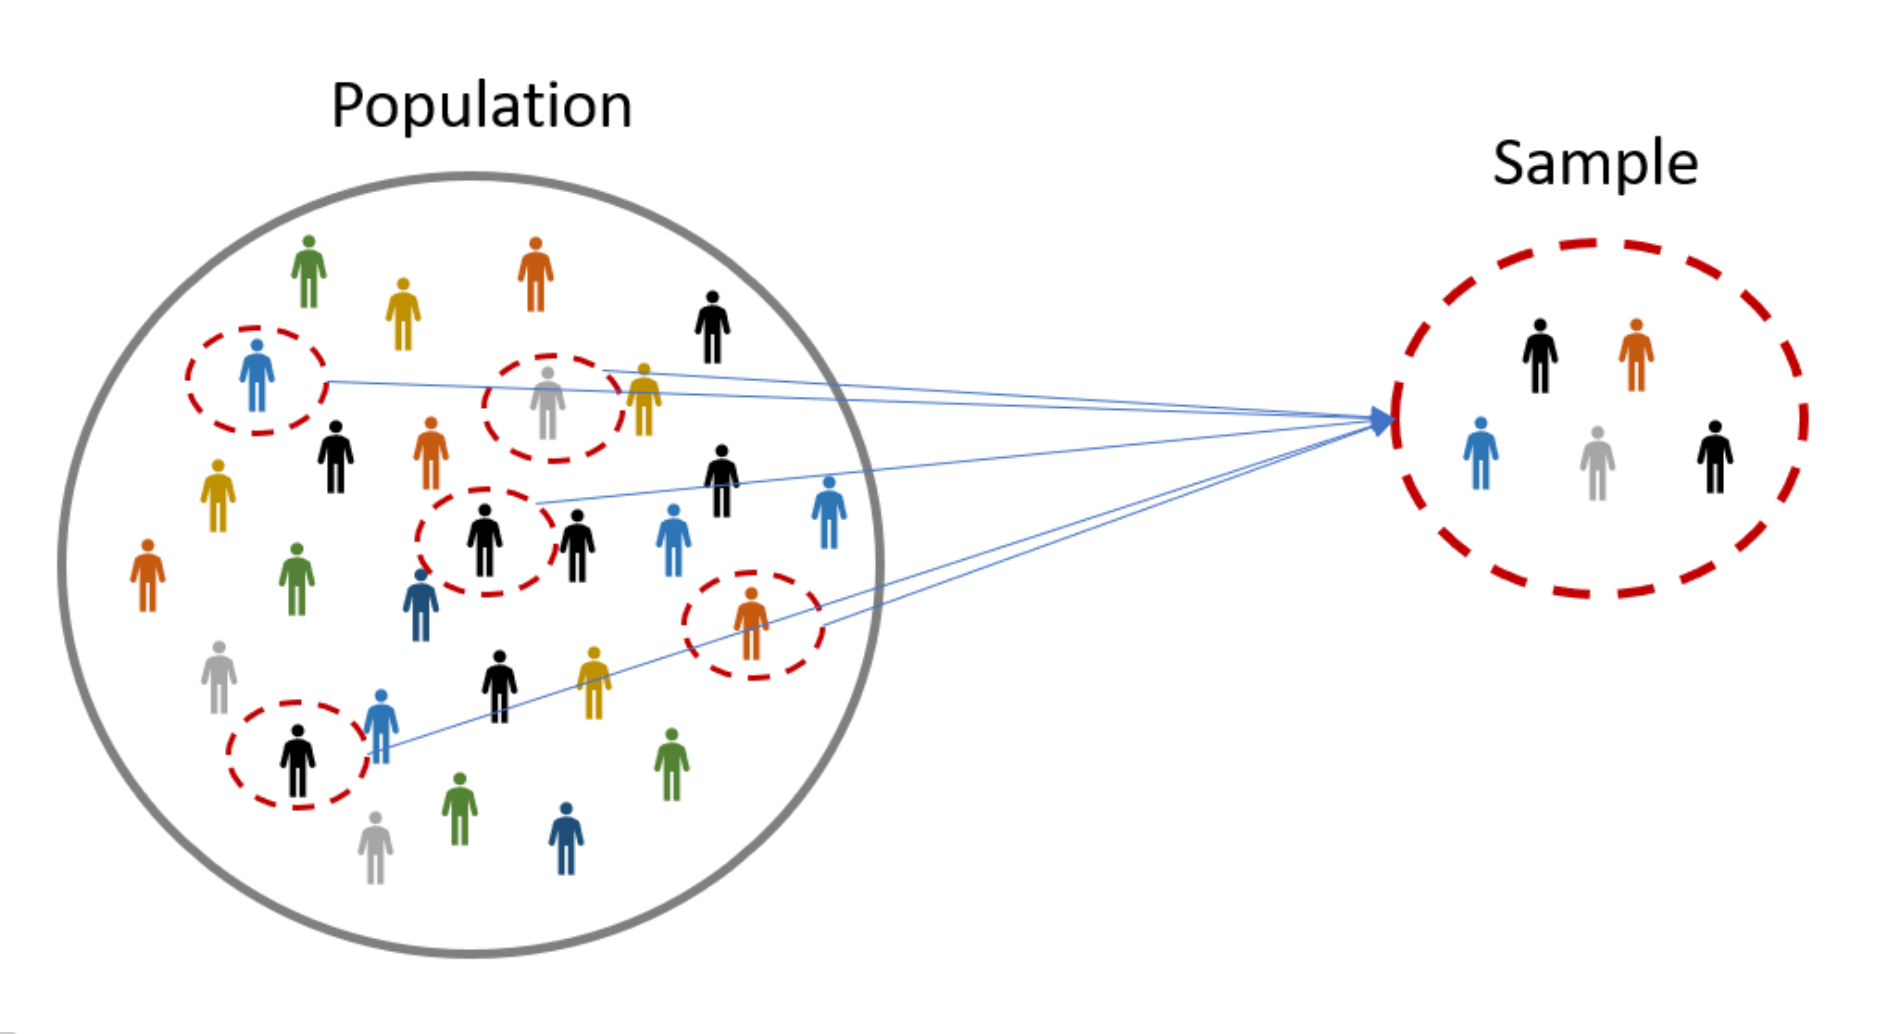
\includegraphics[width=.8\textwidth]{popsamp}
%   \end{center}

%   \pause

  
% \end{frame}

\section{Probability distribution of r.v.}
\begin{frame}
  \frametitle{Probability distribution}
  \pause

  A probability distribution governs the values of a random variable.\\ \pause

  It can be described by the following functions: \pause

  \begin{itemize}[<+->]
  \item probability mass function, PMF \pause {\og discrete random variable} \pause
  \item probability density function, PDF \pause {\og continuous random variable} \pause
  \item cumulative distribution function, CDF \pause {\og discrete/continuous random variable}
  \end{itemize}
\end{frame}

\begin{frame}{Cumulative distribution function (CDF)}
  The CDF ($F_X$) of a random variable $X$ is given by\pause

  \begin{equation}
    \label{eq:11}
    F_X \pause \equiv \pause P(X\le x) \pause \quad \text{for all } x
  \end{equation}
  \pause

  The CDF satisfies the basic axioms of probability:\pause

  \begin{enumerate}[<+->]
  \item      $F_X(-\infty) = 0$ and    $ F_X(\infty) = 1 $

  \item $F_X(x) \ge 0 \quad \forall x$ and is nondecreasing with $x$.\footnote{  Note that the symbol $\forall$ means ``for all''
}

  \item $F_X(x)$ is continuous to the right with $x$.
  \end{enumerate}
  \pause

\end{frame}

\begin{frame}
  \frametitle{Probability mass function (PMF)}\pause
  \begin{minipage}{.45\linewidth}
  The PMF is given by \pause

  \begin{equation}
    \label{eq:12}
    p_X(x_i) \equiv P(X = x_i) \quad \forall x
  \end{equation}

  \pause
  
  \begin{alertblock}{CDF of discrete random variable}
    \pause
    \begin{eqnarray*}
      \label{eq:14}
      F_X(x) &=&\sum_{x_i \le x} P(X = x_i)\\
             &=&\sum_{x_i \le x}p_X(x_i)
    \end{eqnarray*}
  \end{alertblock}
  \end{minipage}\qquad
  \begin{minipage}{.45\linewidth}
    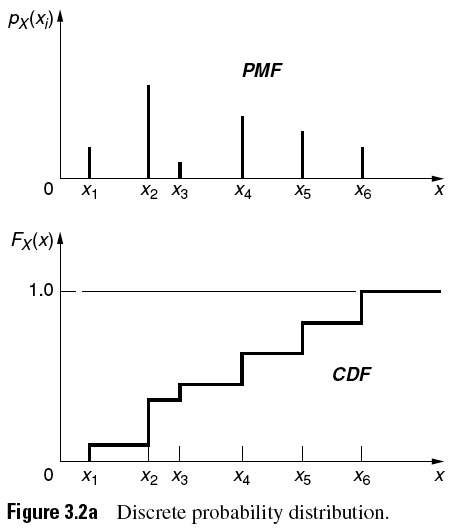
\includegraphics[width=\textwidth, trim={0 1cm 0 0}, clip]{03_02a}
  \end{minipage}
  
  \pause

  The probability masses in a PMF sum up to 1.
\end{frame}

\begin{frame}
  \frametitle{Probability density function (PDF)}\pause

  The PDF is denoted $f_X(x)$ such that the probability of $X$ in the interval $(a,b]$ is: \pause

  \begin{equation}
    \label{eq:10}
    P(a< X \le b) = \int_a^b f_X(x)dx
  \end{equation}

  \pause
  
  \begin{alertblock}{CDF of continuous random variable}
    \pause
    \begin{eqnarray*}
      \label{eq:15}
      F_X(x) &=& P(X \le x)\\
             &=&\int_{-\infty}^x f_X(\tau)d\tau
    \end{eqnarray*}
  \end{alertblock}

    \pause

    It follows that the PDF is the derivative of the CDF:

    \begin{equation}
      \label{eq:15}
      f_X(x) = \fr{dF_X(x)}{dx}
    \end{equation}
  
\end{frame}

\begin{frame}
  \frametitle{PDF (cont.)}
  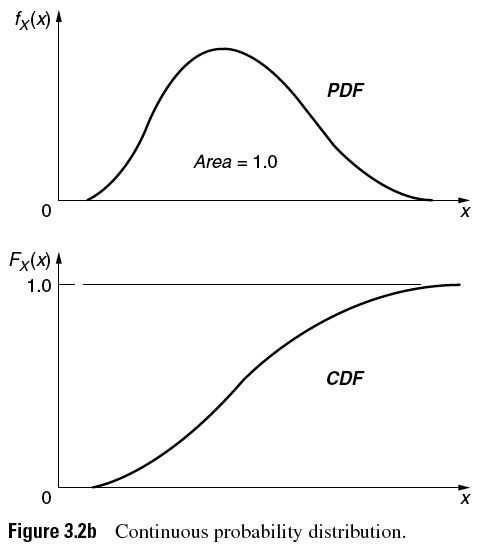
\includegraphics[width=.6\textwidth, trim={0 2cm 0 0}, clip]{03_02b}
  \pause
  
  The total area under a PDF is 1.
\end{frame}

\begin{frame}
  \frametitle{Further derivations}

  \begin{enumerate}[<+->]
  \item Continuous case:
    \begin{equation}
      \label{eq:21}
      P(a < X \le b) = \int_{-\infty}^b f_X(x)dx  - \int_{-\infty}^a f_X(x)dx
    \end{equation}

  \item Discrete case:

    \begin{equation}
      \label{eq:22}
      P(a < X \le b) = \sum_{x_i \le b} p_X (x_i) - \sum_{x_i \le a} p_X (x_i)
    \end{equation}

  \item For all random variables:

    \begin{equation}
      \label{eq:23}\rd
      P(a < X \le b) = F_X(b) - F_X(a)
    \end{equation}
  \end{enumerate}
\end{frame}


\begin{frame}
  \frametitle{Example 1: Operating condition of bulldozers}
  \begin{minipage}{.5\linewidth}
    Each of 3 bulldozers equally likely to operational or nonoperational after 6 months. \pause
    Plot the PMF and CDF of the random variable $X$ which represents the operating condition of the bulldozers after 6 months.
    \pause

    \medskip

    \begin{itemize}[<+->]
    \item Let the outcomes be $O$ (operational) and $N$ (nonoperational)
    \item There are $2\times 2 \times 2 = 8$ possibilities:
      \begin{enumerate}[<+->]
      \item $\pl OON$
      \item $\bl OOO$
      \item $\pl ONO$
      \item $\gr ONN$
      \item $\pl NOO$
      \item $\gr NON$
      \item $\gr NNO$
      \item $\rd NNN$
      \end{enumerate}
      
    \end{itemize}
    
  \end{minipage}
  \pause
    \begin{minipage}{.45\linewidth}
    \begin{figure}[h!]
      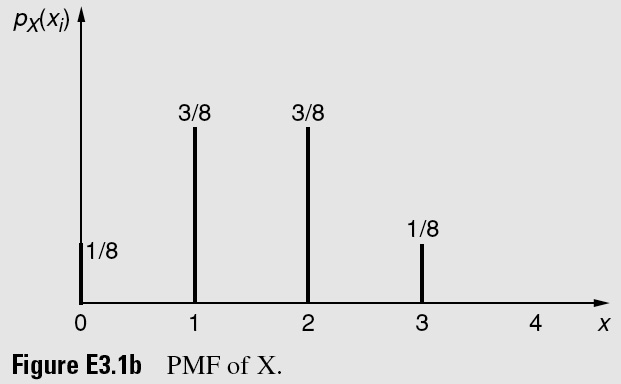
\includegraphics[width=.85\textwidth,trim={0 1.5cm 0 0}, clip ]{E_03_01b}      
      \caption{PMF}
    \end{figure}
    \vspace{-2ex} \pause
    \begin{figure}[h!]
      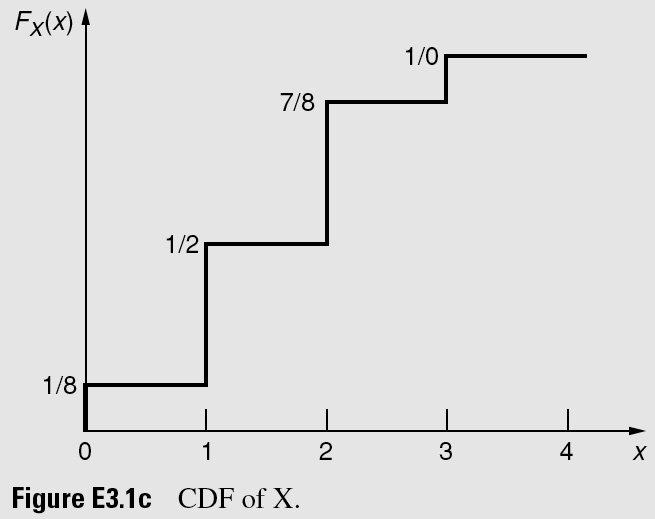
\includegraphics[width=.85\textwidth,trim={0 1.5cm 0 0}, clip ]{E_03_01c}
      \caption{CDF}
    \end{figure}
  \end{minipage}

\end{frame}




\section{Discrete r.v.'s}

\begin{frame}
  \frametitle{Mean and variance} \pause

  \begin{block}{Mean}
     Weighted average or expected value \pause
    \begin{eqnarray}
      E(X) &=&\sum_i x_i p_X(x_i) \quad \text{\og discrete case} \pause
    \end{eqnarray}
  \end{block}
   
  \begin{block}{Variance}\pause
    In the discrete case: \pause
    \begin{equation}
      \label{eq:var}
      Var(X) = \sum_i(x_i - \mu_X)^2p_X(x_i)
    \end{equation}
    \pause

    Expanding  results in:
    
    \begin{equation}
      \label{eq:3}\rd
      Var(X) = E(X^2) - \mu_X^2
    \end{equation}
  \end{block}
\end{frame}



\begin{frame}
  \frametitle{Measures of dispersion (cont.)}
  \pause

  \begin{block}{Standard deviation}
    \pause

    The standard deviation is convenient as it has the same unit as the random variable:\pause

    \begin{equation}
      \label{eq:4}
      \sigma_X = \pause \sqrt{Var(X)}
    \end{equation}
  \end{block}
  
  \pause

  \begin{block}{Coefficient of variation}
    The COV gives the deviation relative to the mean. It is unitless.\pause

    \begin{equation}
      \label{eq:5}
      \delta_X = \frac{\sigma_X}{\mu_X}
    \end{equation}
  \end{block}
  
\end{frame}


\begin{frame}
  \frametitle{Example 2: Bulldozers revisited}
  \pause

  You are given the PMF (probability mass function)
  of the operating condition $X$ of bulldozers after 6 months. 

  \pause

  \begin{center}
  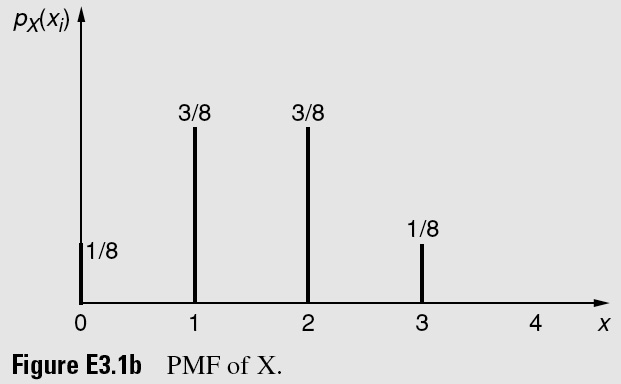
\includegraphics[width=.5\textwidth, trim={0 1.2cm 0 0}, clip]{E_03_01b}
\end{center}

\bigskip
\pause

  Find the mean, variance, standard deviation and coefficient of variation of $X$.

\end{frame}

\begin{frame}
  \frametitle{Example 2: Bulldozers revisited (cont.)}
  \pause
  
    \begin{center}
      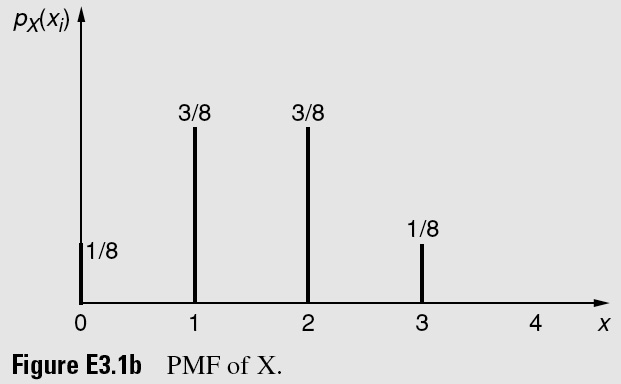
\includegraphics[width=.5\textwidth, trim={0 1.2cm 0 0}, clip]{E_03_01b}
    \end{center}
  \pause
    
    \begin{enumerate}[(a)]
      \item $\mu_X  = E(X) = 0\lt(\fr18\rt) +  1\lt(\fr38\rt) +  2\lt(\fr38\rt) +  3\lt(\fr18\rt) = 1.5$. \pause
      \item $Var(X) = [0^2\lt(\fr18\rt) +  1^2\lt(\fr38\rt) +  2^2\lt(\fr38\rt) +  3^2\lt(\fr18\rt)]  - (1.5)^2 = 0.75$ \pause
      \item $\sigma_X = \sqrt{0.75} = 0.866$ \pause
      \item $\delta_X = \fr{0.866}{1.50} = 0.577$
\end{enumerate}

\end{frame}

\section{Continuous r.v.'s}
\begin{frame}
  \frametitle{Mean and variance} \pause
  These include the mean, median and mode. \pause

  \begin{itemize}[<+->]
  \item Mean: weighted average or expected value \pause
    \begin{eqnarray}
      E(X) &=&\int_{-\infty}^{\infty}xf_X(x)dx \quad \text{\og continuous case}
    \end{eqnarray}
  \end{itemize}

  \begin{block}{Variance}\pause
    In the continuous case:\pause
    \begin{equation}
      \label{eq:2}
      Var(X) = \int_{-\infty}^{\infty}(x - \mu_X)^2 f_X(x)dx
    \end{equation}
    \pause

    Expanding both equations results in:
    
    \begin{equation}
      \label{eq:3}\rd
      Var(X) = E(X^2) - \mu_X^2
    \end{equation}
  \end{block}
\end{frame}



\begin{frame}
  \frametitle{Example 3: Loaded beam} \pause
    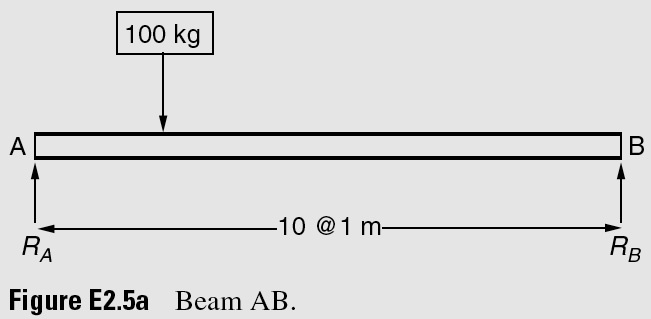
\includegraphics[width=.3\textwidth]{E_02_05a}
    Consider the beam under a 100-kg load. If the load is equally likely to be placed anywhere along the 10m span of the beam,\pause
    then the PDF of the load position $X$ is \alert{uniformly distributed} in $0 < x\le 10$, i.e.:\pause

    \begin{equation}
      \label{eq:e2}
      f_X(c) =
      \begin{cases}
        c & \quad 0 < x \le 10 \\ \pause
        0 & \quad \text{otherwise}
      \end{cases}
    \end{equation}

    \pause

    \begin{enumerate}[(a)]
    \item Plot the PDF of $X$.
    \item Solve the integral for the CDF and plot.
    \item Find $P(2 < X \le 5)$.
    \end{enumerate}
 \end{frame}


\begin{frame}
  \frametitle{Example 3: Loaded beam (cont.)} \pause
    \begin{enumerate}[(a)]
    \item The area under the PDF must be 1. Thus, $c$ must be $\fr1{10}$.\pause
      
      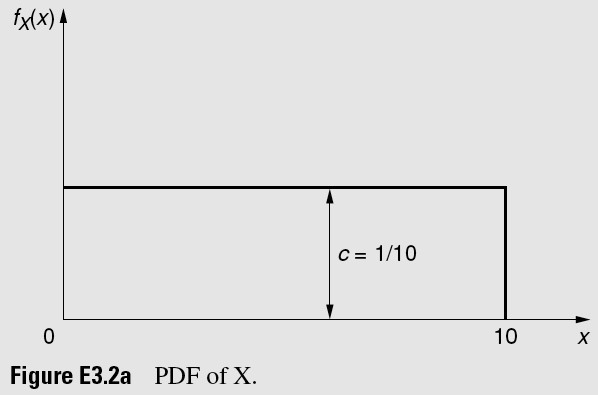
\includegraphics[width=.8\textwidth, trim={0 2cm 0 0}, clip]{E_03_02a}
    \end{enumerate}
 \end{frame}

\begin{frame}
  \frametitle{Example 3: Loaded beam (cont.)} \pause
    \begin{enumerate}[(a)]\setcounter{enumi}{1}
    \item The CDF is given by: \pause
      \begin{eqnarray*}
        F_X &=&\pause \int_0^x cdx \pause =  cx \pause = \fr{x}{10} \qquad \pause 0 < x \le 10
      \end{eqnarray*}
      \pause
      
      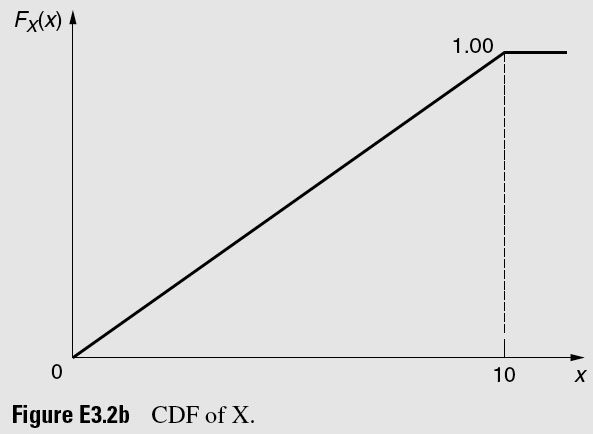
\includegraphics[width=.6\textwidth]{E_03_02b}
    \end{enumerate}
 \end{frame}


\begin{frame}
  \frametitle{Example 3: Loaded beam (cont.)} \pause
  
    \begin{enumerate}[(a)]\setcounter{enumi}{2}
    \item To compute  $P(2 < X \le 5)$, we use the CDF: \pause
      \begin{eqnarray*}
        P(2 < X \le 5) &=& F_X(5) - F_X(2) \\ \pause
                       &=& \fr{5-2}{10}=  \pause 0.3
      \end{eqnarray*}
    \end{enumerate}
 \end{frame}

\begin{frame}
  \frametitle{Example 4: Useful life of machines}
    The useful life $T$ of welding machines is a random variable with an \alert{exponential distribution}. The PDF and CDF are:
    \begin{eqnarray*}
      f_T(t) &=&\lambda e^{-\lambda t} \qquad t\ge 0\\ \pause
      F_T(t) &=&1 - e^{-\lambda t} \qquad t\ge 0
    \end{eqnarray*}
    \pause
    
    \begin{center}
    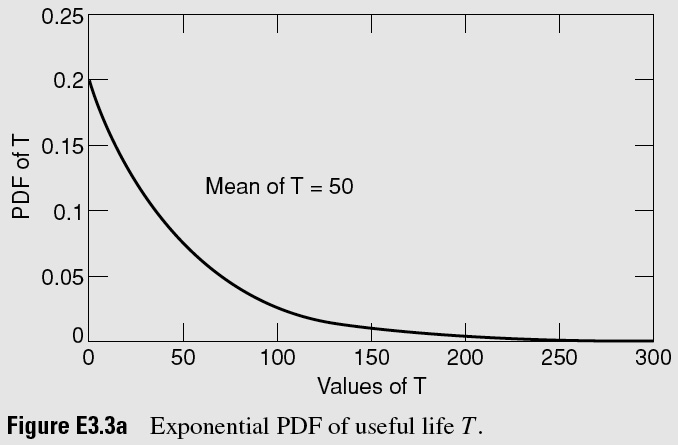
\includegraphics[width=.4\textwidth]{E_03_03a}\quad \pause
    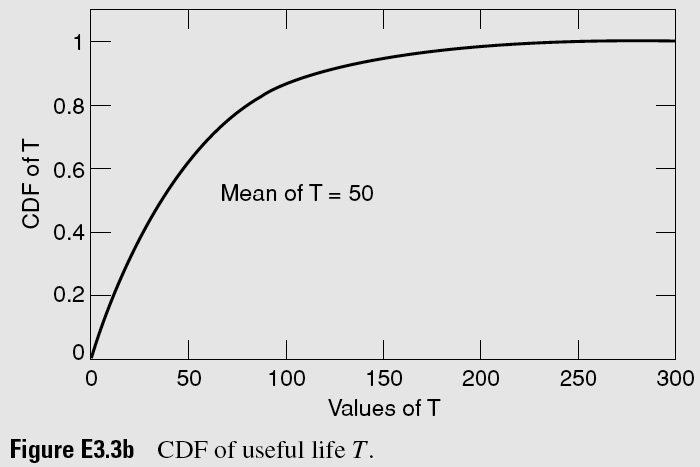
\includegraphics[width=.4\textwidth]{E_03_03b}
  \end{center}
    \pause
    \begin{enumerate}[(a)]
    \item Find the mean of this distribution
    \item Find the median
    \item Show that the variance is $\fr{1}{\lambda^2}$
    \end{enumerate}
 \end{frame}


\begin{frame}
  \frametitle{Example 4: Useful life of machines}
    \begin{eqnarray*}
    \text{PDF}:\pause  f_T(t) &=& \lambda e^{-\lambda t} \qquad t\ge 0\\ \pause
     \text{CDF}:\pause   F_T(t) &=& 1 - e^{-\lambda t} \qquad t\ge 0
    \end{eqnarray*}
    \pause
    \begin{enumerate}[(a)]
    \item The mean is given by $\mu_T = E(T) = \int_0^\infty t\lambda e^{-\la t}dt$.\pause We use integration by parts: $\int u dv = uv - \int v du$.\pause
      \begin{eqnarray*}
        \mu_T &=& \int_0^\infty t\lambda e^{-\la t}dt \\ \pause
              &=& \la \int_0^\infty {\bl \lambda} {\rd  e^{-\la t}dt } \\ \pause
              &=& \la \lt[ \bl t \lt(-\fr{1}{\la} e^{-\la t}\rt) \rt]_0^\infty - {\rd \lt[ -\fr{1}{\la} e^{-\la t} dt \rt] } \\ \pause
              &=& \la \lt( {\bl 0} + {\rd \fr{1}{\la}\fr{-e^{-\la t}}{\la} \Bigl|_0^\infty} \rt) \pause = \fr\la{\la^2} = \fr1\la
      \end{eqnarray*}
    \end{enumerate}
 \end{frame}

 
\section{Outlook}

 
\begin{frame}
  \frametitle{Recap}
  \begin{itemize}[<+->]
  \item Random variables
  \item Probability mass/density function (PMF/PDF) and cumulative distribution function (CDF)
  \item Measures of centrality
  \item Measures of dispersion
  \end{itemize}

  \begin{block}{Reading}
    \begin{itemize}
    \item  Open Intro Statistics Section 3.4 (Random variables)
    \item Open Intro Statistics Section 3.5 (Continuous distributions)
    %   Navidi: Section 2.4 (Random Variables)
    % \item Supplementary Reading: Open Intro Statistics Section 3.4 (Random variables)
    \end{itemize}
  \end{block}
\end{frame}




%\backupbegin
\section{Appendix}



\begin{frame}
  \frametitle{Skewness}\pause
  The skewness or symmetry of a distribution is measured by the third central moment: \pause

  In the discrete case: \pause
    \begin{equation}
      \label{eq:var}
      E(X - \mu_X)^3 = \sum_i(x_i - \mu_X)^3p_X(x_i)
    \end{equation}
    \pause

    In the continuous case:\pause
    \begin{equation}
      \label{eq:6}
      E(X - \mu_X)^3 = \int_{-\infty}^{\infty}(x - \mu_X)^3 f_X(x)dx
    \end{equation}

    \pause

    For convenience, the skewness coefficient is also used (unitless):\pause

    \begin{equation}
      \label{eq:7}
      \theta = \fr{E(X - \mu_X)^3}{\sigma^3}
    \end{equation}
    
\end{frame}

\begin{frame}
  \frametitle{Skewness (cont.)}
  \pause

  \begin{itemize}[<+->]
  \item Positive skewness is characterized by a long right tail (right-skewed)
  \item Negative skewness is characterized by a long left tail (left-skewed)
  \end{itemize}

  \pause

  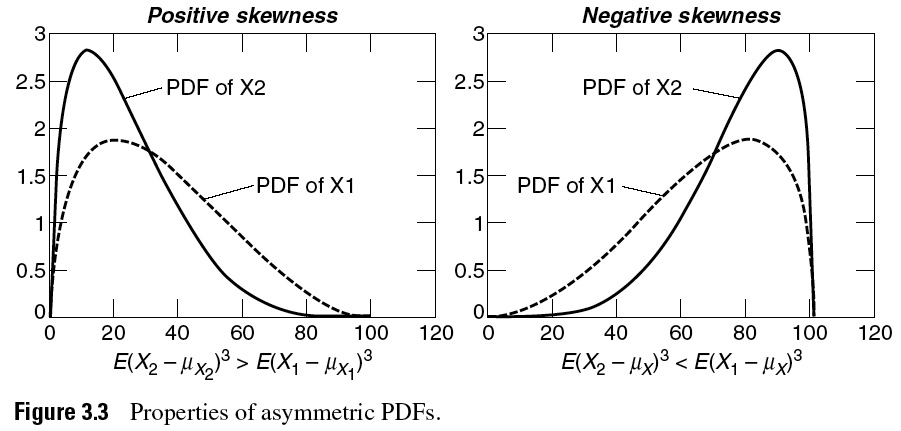
\includegraphics[width=\textwidth,trim={0 2cm 0 0},clip]{03_03}
  
\end{frame}
\begin{frame}
  \frametitle{Kurtosis} \pause

  This is the measure of peakedness in a distribution. \pause It is the fourth central moment: \pause

  
  In the discrete case: \pause
    \begin{equation}
      \label{eq:8}
      E(X - \mu_X)^4 = \sum_i(x_i - \mu_X)^4p_X(x_i)
    \end{equation}
    \pause

    In the continuous case:\pause
    \begin{equation}
      \label{eq:6}
      E(X - \mu_X)^4 = \int_{-\infty}^{\infty}(x - \mu_X)^4 f_X(x)dx
    \end{equation}


\end{frame}

\begin{frame}
  \frametitle{Skewness vs. kurtosis}
  \pause

  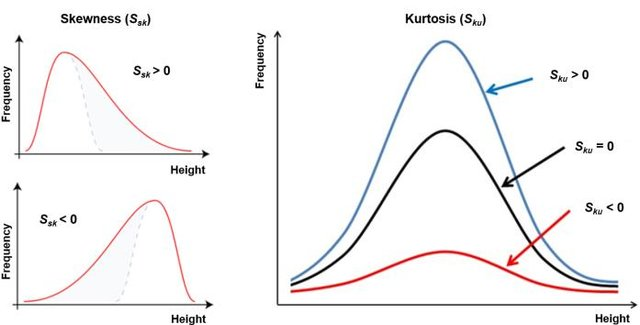
\includegraphics[width=\textwidth]{skewness-kurtosis}

  {\tiny Source: Bonyar, A (2015) ``Application of localization factor for the detection of tin oxidation with AFM'' DOI: 10.1109/SIITME.2015.7342289}
\end{frame}

\begin{frame}
  \frametitle{Generalized expectation}
  The mathematical expectation can be defined for a function $g$ of random variable $X$:
  
     \begin{eqnarray}
      E[g(X)] &=&\sum_i g(x_i) p_X(x_i) \quad \text{\og discrete case}\\ \pause
      E[g(X)] &=&\int_{-\infty}^{\infty}g(x)f_X(x)dx \quad \text{\og continuous case}
    \end{eqnarray}

  \end{frame}
  

%\backupend

%\begin{frame}[allowframebreaks]
%   \frametitle{References}
%   \AtNextBibliography{\scriptsize}
%   \setbeamertemplate{bibliography item}[text]
%   \printbibliography[heading=none]
  
% \end{frame}

%\printbibliography
\end{document}
%%% Local Variables:
%%% mode: latex
%%% TeX-master: t
%%% End:
